\chapter{Interacțiunea cu mediul extern}

\section{Senzori cu infraroșu}

Pentru a putea detecta diferența dintre linia neagră și fundalul alb al traseului, robotul \textit{Zumo} folosește o matrice de senzori cu infraroșu. Acești senzori pot măsura cantitatea de lumina reflectată de diferite suprafațe, în funcție de proprietățile acesteia. Cum funcționează? Foarte simplu. O diodă emite radiații în spectrul infraroșu spre suprafața din dreptul senzorului și o parte mai mică sau mai mare din această lumina va fi absorbită de suprafață. Ce ne interesează pe noi este cantitea de lumina reflectată ce va fi masurată cu ajutorul unui fototranzistor și al unui condensator.

\begin{wrapfigure}{l}{0.5\textwidth}
    \vspace{-20pt}
    \center{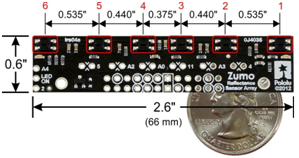
\includegraphics[width=0.5 \textwidth]{images/InfraredSensors.png}}
    \vspace{-15pt}
    \caption{\label{fig:CodeWarrior-InfraredSensors} Bareta de senzori}
    \vspace{-20pt}
\end{wrapfigure}

După cum îi spune și numele, matricea de senzori este alcătuită din mai multe elemente. Acest lucru este necesar deoarece fiecare senzor poate măsura doar cantitatea de lumina care este reflectată din jurul său (pe o arie redusă ca și suprafață). Bareta care este pusă la dispoziție pentru robotul Zumo are 6 astfel de elemente pentru detecția liniei negre. Aceasta este amplasată sub lama robotului, asigurându-se o protecție atât mecanică cât și o reducere a cantității de lumina ambientală care poate duce la perturbarea măsurătorilor.

Ieșirea senzorilor este dată de durata ($T$) a unui impuls electric. Cu cât impulsul este mai de durată, cu atât cantitatea de lumina reflectată este mai mică.

Următoarele componente \textit{Processor Expert} vor fi folosite în interfațarea cu acești senzori:

\begin{itemize}
    \item intrările / ieșirile digitale (componente de tip \textit{BitIO}): A1, A3, D11, A0, A2, D5, IR\_LED;
    \item un timer (componentă de tip \textit{TimerUnit\_LDD}) CountTimer;
    \item componentă necesară adăugării unui întârzieri - \textit{WAIT1};
\end{itemize}

Pașii necesari pentru obținerea unei iterații de date despre mediu, de la senzori, ar fi următorii:

\begin{enumerate}
    \item Activăm diodele infraroșii - IR\_LED.
    \item Configurăm pinii digitali (A1, A3, D11, A0, A2, D5) ca ieșiri și le setăm pe valoarea 1.
    \item Așteptăm o perioadă de timp astfel încât condensatorul să se încarce - 50 µs este suficient.
    \item Configurăm pinii de la pasul 2 ca intrări digitale, de această dată.
    \item Resetăm timer-ul \textit{CountTimer}. După inițializare acestă funcționează în continuu astfel avem nevoie de o resetare a timpului măsurat până atunci – nu se știe starea în care va fi găsit. Timer-ul măsoară perioade de timp în multipli de 6.10 µs (163.84kHz).
    \item Măsurăm timpul necesar ca tensiunea de pe condensator să comute intrările în valoarea 0. După o perioadă de câteva µs, senzorii pot fi considerați ca au toți valoarea 0. Acest mecanism ne permite să reducem perioada de așteptare între citiri, după un anumit prag (perioadă) nu se mai obține informatii utile de la senzori.
    \item Dezactivăm diodele infraroșii.
\end{enumerate}